\documentclass[border=2mm]{standalone}

\usepackage{tikz}
\usetikzlibrary{decorations.pathreplacing}

\definecolor{myLightGray}{RGB}{191,191,191}
\definecolor{myGray}{RGB}{160,160,160}
\definecolor{myDarkGray}{RGB}{144,144,144}
\definecolor{myDarkRed}{RGB}{167,114,115}
\definecolor{myRed}{RGB}{255,58,70}
\definecolor{myGreen}{RGB}{0,255,71}

\begin{document}

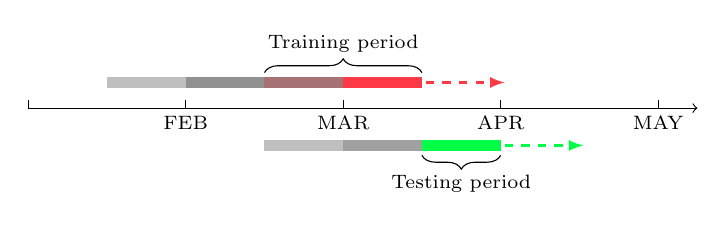
\begin{tikzpicture}[%
    every node/.style={
        font=\scriptsize,
        % Better alignment, see https://tex.stackexchange.com/questions/315075
        text height=1ex,
        text depth=.25ex,
    },
]
% draw horizontal line   
\draw[->] (0,0) -- (8.5,0);

% draw vertical lines
\foreach \x in {0,2,4,6,8}{
    \draw (\x cm,3pt) -- (\x cm,0pt);
}

% place axis labels
\node[anchor=north] at (2,0) {FEB};
\node[anchor=north] at (4,0) {MAR};
\node[anchor=north] at (6,0) {APR};
\node[anchor=north] at (8,0) {MAY};

% draw scale above
\fill[myLightGray] (1,0.25) rectangle (2,0.4);
\fill[myDarkGray] (2,0.25) rectangle (3,0.4);
\fill[myDarkRed] (3,0.25) rectangle (4,0.4);
\fill[myRed] (4,0.25) rectangle (5,0.4);
\draw[myRed,dashed,thick,-latex] (5.05,0.325) -- (6.05,0.325);

% draw scale below
\fill[myLightGray] (3,-0.4) rectangle (4,-0.55);
\fill[myGray] (4,-0.4) rectangle (5,-0.55);
\fill[myGreen] (5,-0.4) rectangle (6,-0.55);
\draw[myGreen,dashed,thick,-latex] (6.05,-0.475) -- (7.05,-0.475);

% draw curly braces and add their labels
\draw[decorate,decoration={brace,amplitude=5pt}] (3,0.45) -- (5,0.45)
    node[anchor=south,midway,above=4pt] {Training period};
\draw[decorate,decoration={brace,amplitude=5pt}] (6,-0.6) -- (5,-0.6)
    node[anchor=north,midway,below=4pt] {Testing period};
\end{tikzpicture}

\end{document}